\section{BALANCED SCORE CARD} 

\subsection{ DESCRIPCION DEL BALANCED SCORECARD}

	El Balanced Scorecard (BSC) o Cuadro de Mando Integral es un modelo de planificación y gestión que permite alinear a la 			organización con su estrategia. Traduce la estrategia en objetivos relacionados, medidos a través de indicadores y ligados a unos 		planes de acción que permiten alinear el comportamiento de los miembros de la organización.

	Aspectos Claves:
	
	\begin{itemize}
	
		\item  Modelo simple que priorice lo importante
		\item  Utilización de un lenguaje común
		\item  Equipo líder
		\item  Buena comunicación
		\item  Participación de diferentes personas de la organización

	\end{itemize}

	La utilidad del Balanced Scorecard no depende del tipo de empresa, sino de los problemas a los que se enfrenta. El Cuadro de 			Mando Integral se ha implantado en empresas grandes y pequeñas en sectores regulados y no regulados, en organizaciones con 		y sin ánimo de lucro; así como, en empresas con alta rentabilidad y con pérdidas. El cambio depende de nuestro grado de 			satisfacción con el actual modelo de gestión y con la comprensión de la estrategia de la empresa que demuestran las personas de 		nuestra organización.

	A continuación se muestra en un gráfico las fases del Balanced Scorecard.

			\begin{figure}[htb]
				\begin{center}
					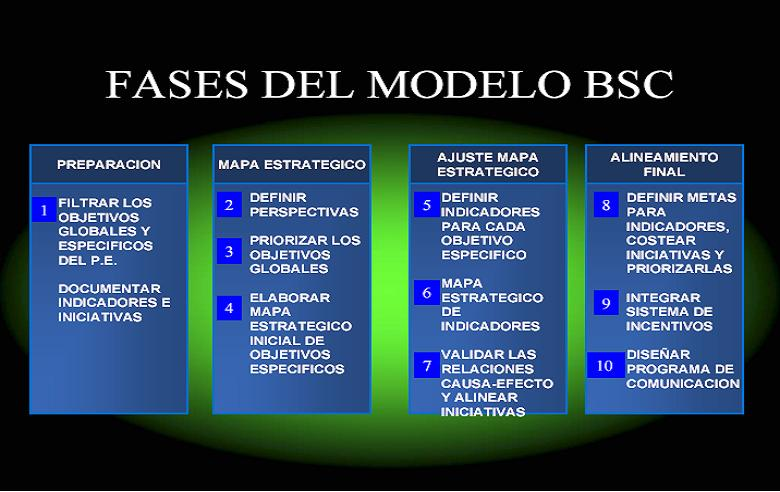
\includegraphics[width=10cm]{./Imagenes/1}
				\end{center}
			\end{figure}

	El Balanced Scorecard no es un reporte de resultados; es un vehículo de comunicación de la estrategia y visión de la compañía. En 		ese sentido, para lograr el éxito en la implementación de la filosofía del BSC se requiere tener el apoyo de los líderes de la 			empresa, quienes deben cumplir los pasos siguientes:

	\begin{itemize}

	\item 	Tener compromiso.
	\item  Crear un modelo de BSC con sus objetivos estratégicos e indicadores clave de desempeño
	\item  Educar al personal, de manera que el BSC sea parte de la cultura organizacional.
	\item  Tener soporte tecnológico (software), en caso no se tenga los recursos necesarios para comprar un software especializado en el tema, se puede utilizar el excel por ser un software muy común en las empresas y contar con herramientas aprovechables en el diseño de formatos para el control del BSC durante la fase de puesta en práctica.
	\end{itemize}

	Es un poderoso instrumento para medir el desempeño corporativo y se ha demostrado que es la herramienta más efectiva para enlazar la visión y la estrategia a cuatro medidas de desempeño, que son:

	\begin{itemize}
		\item Resultados financieros.
		\item Satisfacción de clientes (Internos y externos).
		\item Operación Interna (procesos).
		\item Creatividad, innovación, satisfacción y desarrollo de competencias de los empleados

	\end{itemize}

\subsection{ ELEMENTOS DEL BALANCED SCORECARD}

	Los elementos que conforman el Balanced Scorecard son: el foco estratégico, perspectivas, mapa estratégico, indicadores, metas, iniciativas y responsables de  objetivos o iniciativas.

	\begin{enumerate}[a)]
       	 \item Foco Estratégico o propuesta de valor al cliente
		Selección de aquellos objetivos estratégicos de primer nivel que son prioritarios y que diferenciarán a nuestra organización ante los clientes.

Los focos estratégicos son:

		\begin{itemize}

 		\item[$*$] Liderazgo en Costos: Proporcionar productos y servicios a un precio competitivo para la calidad y funcionalidad que ofrecen.
		\item[$*$] Liderazgo en Producto o Servicios: Se centra en la excelencia de sus productos y servicios, que ofrecen la máxima calidad y funcionalidad.
		\item[$*$] Intimidad con el Cliente: Capacidad de generar vínculos con los clientes para conocerlos y proporcionarles productos y servicios adecuados a sus medidas.

		\end{itemize}

	A continuación se muestra un gráfico en el cual se presenta cada uno de los focos con los temas que estos incluyen.

			\begin{figure}[htb]
				\begin{center}
					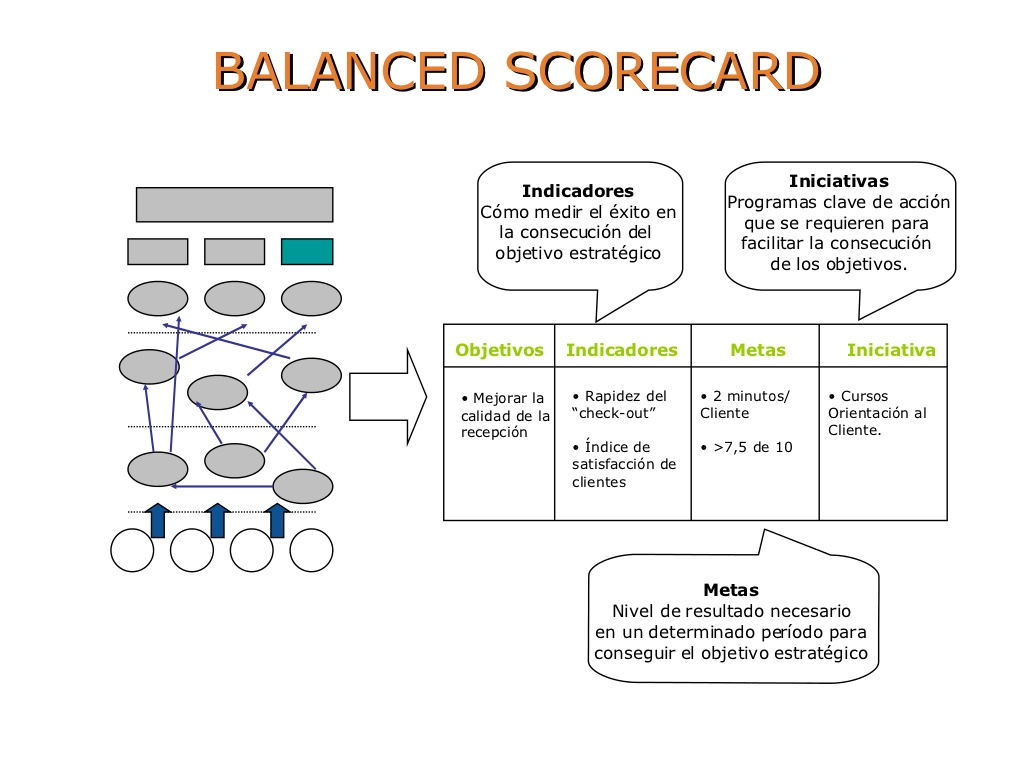
\includegraphics[width=10cm]{./Imagenes/2}
				\end{center}
			\end{figure}


        \item Mapa Estratégico en Balanced ScoreCard
	Llamamos mapa estratégico al conjunto de objetivos estratégicos que se conectan a través de relaciones causales.
El mapa estratégico ayuda a valorar la importancia de cada objetivo estratégico, ya que nos los presenta agrupados en perspectivas. Las perspectivas son aquellas dimensiones críticas clave en la organización. A continuación, se detallarán las cuatro perspectivas.

		\begin{enumerate}[1.]
   		 \item Perspectiva Financiera en Balanced ScoreCard

		Las medidas de actuación financiera indican si la estrategia de una empresa, su puesta en práctica y ejecución, están contribuyendo a la mejora del mínimo aceptable. Los objetivos financieros acostumbran a relacionarse con la rentabilidad, medida, por ejemplo, por los ingresos de explotación, los rendimientos del capital empleado, o más recientemente por el valor añadido económico. Otros objetivos financieros pueden ser el rápido crecimiento de las ventas o la generación de cash flow (flujo de caja). Esta definición se puede resumir en la siguiente pregunta: ¿Qué debemos hacer para satisfacer las expectativas de nuestros accionistas?

  		 \item Perspectiva del Cliente en Balanced ScoreCard

		Identifica los segmentos de clientes y mercado donde se va a competir; así como, mide las propuestas de valor que se orientan a los clientes y mercados. Evalúa las necesidades de los clientes, satisfacción, lealtad, adquisición y rentabilidad; con el fin de alinear los productos y servicios con sus preferencias. Traduce la estrategia y visión en objetivos sobre clientes y segmentos siendo estos los que definen los procesos de marketing, operaciones, logística, productos y servicios.
Entre los principales objetivos que se manejan en esta perspectiva podemos señalar los siguientes: volúmenes de clientes (participación en el mercado y adquisición de nuevos clientes), satisfacción y fidelización de los clientes. Los objetivos de esta perspectiva se pueden resumir en la siguiente pregunta: ¿Qué debemos hacer para satisfacer las necesidades de nuestros clientes?

  		  \item Perspectiva Interna en Balanced ScoreCard

		Define la cadena de valor de los procesos necesarios para entregar a los clientes soluciones a sus necesidades (innovación, operación y servicio de post venta). Los objetivos e indicadores de esta perspectiva se derivan de estrategias explícitas para satisfacer las expectativas de los clientes.
Se identifican los objetivos e indicadores estratégicos asociados a los procesos clave de la organización o expectativas de clientes y accionistas. Usualmente, esta perspectiva se desarrolla luego que se han definido los objetivos e indicadores de las perspectivas financiera y cliente. Los indicadores de esta perspectiva deben manifestar la naturaleza misma de los procesos propios de la empresa u organización. Los objetivos de esta perspectiva se pueden resumir en la siguiente pregunta: ¿En qué procesos debemos ser excelentes para satisfacer esas necesidades?

		\item Perspectiva de Aprendizaje y Crecimiento en Balanced ScoreCard

		En esta perspectiva se obtienen los inductores necesarios para lograr resultados en las anteriores perspectivas. La formación y crecimiento de una organización proceden de tres fuentes principales: las personas, los sistemas y los procedimientos de la organización.
La actuación del personal se refuerza con agentes motivadores que estimulen sus intereses hacia la empresa. Se mide en esta perspectiva las capacidades (competencias, creatividad, innovación, entre otros) de los empleados, las capacidades de los sistemas de información, y el clima organizacional para medir la motivación y las iniciativas del personal.


		\end{enumerate}

	 \item Indicadores y las Metas en Balanced ScoreCard

	Los indicadores (también llamados medidas) son el medio que tenemos para visualizar si estamos cumpliendo o no los objetivos estratégicos.
Un objetivo estratégico como por ejemplo el desarrollo de capacidades comerciales del personal clave, puede medirse a través de indicadores. No existen indicadores perfectos, y por eso, para la medición de algunos objetivos estratégicos, se puede utilizar más de uno. Por ejemplo, el desarrollo de esas capacidades comerciales se puede medir a través de indicadores como el número de horas de formación por persona, el índice de satisfacción de los empleados con la formación percibida o el incremento medio de los contratos o ingresos por empleado. Se puede establecer dos tipos de indicadores:

		\begin{itemize}
  		  \item Indicadores de Resultado:Los indicadores de resultado denotan la conclusión de varias acciones tomadas y medidas, la información que dan es definitiva. Mide el éxito en el logro de los objetivos del BSC sobre un período específico de tiempo. Se usan para reportar el desempeño de la organización en la implantación de su estrategia. Para cada indicador como es habitual se debe fijar metas, como regla general debieran ser metas ambiciosas pero posibles de ser logradas.

  		  \item Indicadores de Causa u Operativos: Los indicadores de causa u operativos indican a futuro cual puede ser el resultado de un grupo de acciones u operaciones definidas en un indicador de resultado también se le denomina indicadores inductores de actuación. Provee indicación temprana del progreso hacia el logro de los objetivos; su propósitos es generar los comportamientos adecuados para el logro de la estrategia. Usualmente miden lo que debe “hacerse bien” para alcanzar los objetivos. Miden las palancas de valor, los elementos “impulsores” del desempeño. Su propósito es canalizar y direccionar esfuerzos. También llamados Inductores de Actuación.
  		 
    
 		  \end{itemize}


	 \item Iniciativas Estratégicas en Balanced ScoreCard
		Las iniciativas estratégicas son las acciones en las que la organización se va a centrar para la consecución de los objetivos estratégicos. Es importante priorizar las iniciativas en función de los objetivos estratégicos. Si analizamos el impacto de las iniciativas en marcha en cada uno de los objetivos estratégicos, podremos visualizar: iniciativas que aportan poco valor al cumplimiento de esos objetivos y objetivos sin soporte en las iniciativas. Las iniciativas pueden tener sus propios indicadores para el seguimiento e incluso un Balanced Scorecard propio.

	\item Responsables y Recursos en Balanced ScoreCard
		Cada objetivo, indicador e iniciativa debe tener su responsable. Una persona a cargo que controla su cumplimiento.
Otro aspecto clave para una implantación con éxito del Balanced Scorecard es asignar los recursos necesarios para el buen desarrollo de las iniciativas estratégicas. Por ello es necesario establecer los equipos a cargo de cada iniciativa; así como, el papel que diferentes personas van a jugar en ellos. Y también dotar a las iniciativas de los recursos necesarios para su cumplimiento. Se recomienda que el presupuesto contenga una partida de recursos asignados a las iniciativas, estos recursos deben estar diferenciados del presupuesto operativo, del presupuesto de inversiones y otros presupuestos.

    \end{enumerate}


\subsection{ BENEFICIOS DEL BALANCED SCORECARD}

	Los Beneficios de implementar el Balanced Scorecard son:

	\begin{itemize}
   	 \item Comunicar la visión y estrategia a toda la organización.
	\item Traducir objetivos estratégicos y tácticos de la organización en medidas individuales de rendimiento y productividad.
	\item Ofrecer a cada empleado su contribución individual al logro de los objetivos de la empresa.
	\item Ligar los resultados con los procesos que se desarrollaron en el logro de los mismos.
	\item Alinear las estrategias de la empresa con las competencias requeridas del personal.
	\item Monitorear los recursos necesarios para el logro de objetivos.
	\item Elevar los niveles de servicio a clientes internos y externos.
  	 \end{itemize}